A Tritium-IFIC-2 prototype of $800$ fibers of $1~\mm$ diameter arranged and uniformly distributed in sixteen different layers of increasing radius, as illustrated in Figure \ref{fig:FibersTritiumIFIC2Simulation}, was simulated.

\begin{figure}[h]
\centering
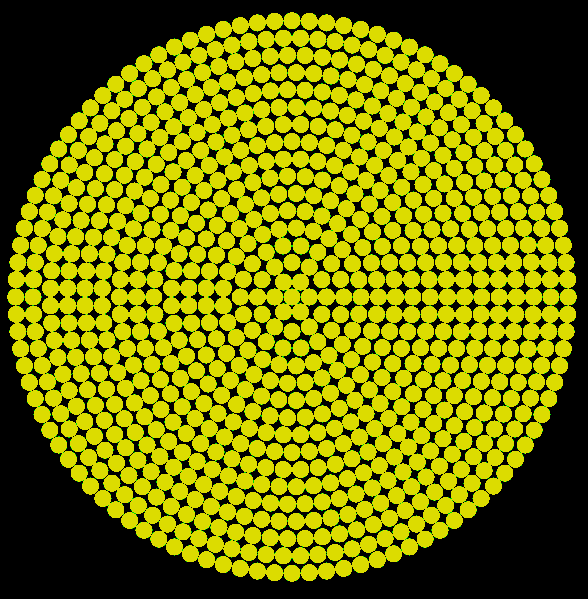
\includegraphics[scale=0.4]{6Simulations/62TRITIUMMonitor/621TRITIUMIFIC2/FiberDistribution_Tritium_IFIC_2_simulation.png}
\caption{Distribution of the scintillating fibers in the simulations of the Tritium-IFIC-2 prototype.\label{fig:FibersTritiumIFIC2Simulation}}
\end{figure}
The tritiated water source consisted of a tritiated water volume of $5~\mu\meter$ thickness around each fiber. Scintillating fibers were located in a cylindrical PTFE vessel. Two PMMA windows of $5~\mm$ thickness closed of both ends. A $0.5~\mm$ layer of optical grease on each PMMA window was included. Two R8520-460 PMTs from Hamamatsu \cite{DataSheetPMTs} were simulated as photosensors. 

%The optical properties used for the tritiated water, PTFE vessel, PMMA windows and the optical grease, mentioned in section \ref{sec:Geant4Environment}, are included in this simulation. 

The inner part of the simulated TRITIUM-IFIC-2 geometry is shown in Figure \ref{fig:TritiumIFIC2Simulation} in which the PMTs (black), the optical grease (blue), the PMMA windows (white), the tritiated water (green) and the scintillating fibers (yellow) are shown. The PMTs do not cover the entire active area formed by the scintillating fiber bundle, preventing phtons of being detected, which slightly reduces the efficiency of the detector.
\begin{figure}[h]
\centering
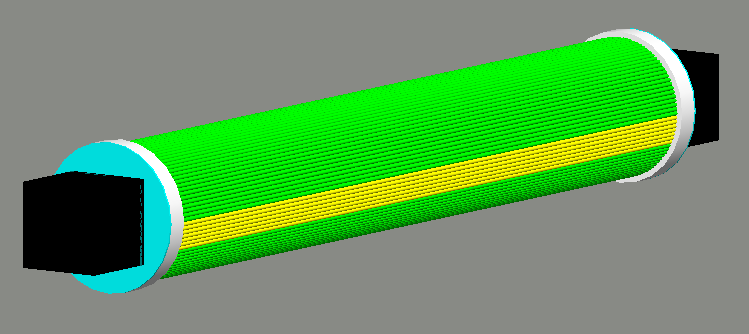
\includegraphics[scale=0.4]{6Simulations/62TRITIUMMonitor/621TRITIUMIFIC2/SimulationTritiumIFIC2.png}
\caption{Simulation of inner part of the Tritium-IFIC-2 prototype. PMTs (black), the optical grease (blue), PMMA windows (white), tritiated water (green) and scintillating fibers (yellow). \label{fig:TritiumIFIC2Simulation}}
\end{figure}
The aim of these simulations was to calculate the activity resolution of the prototype and the improvement by increasing the integration time window and the number of modules read out in parallel. The detection of a tritium electron in TRITIUM-IFIC-2 is shown in Figure \ref{fig:TritiumEventDetectedInSimulatedPrototype}. The paths of the photons created in scintillating fibers are represented by green lines ending in red dots when they are absorbed in the fiber or the water and blue dots when they are absorbed in the PMTs (detected). The fiber in which the tritium electron is detected is clearly identified. Some photons go out of the fiber and are not collected. Blue dots in both PMTs indicate that photons are detected in coincidence.

\begin{figure}[hbtp]
\centering
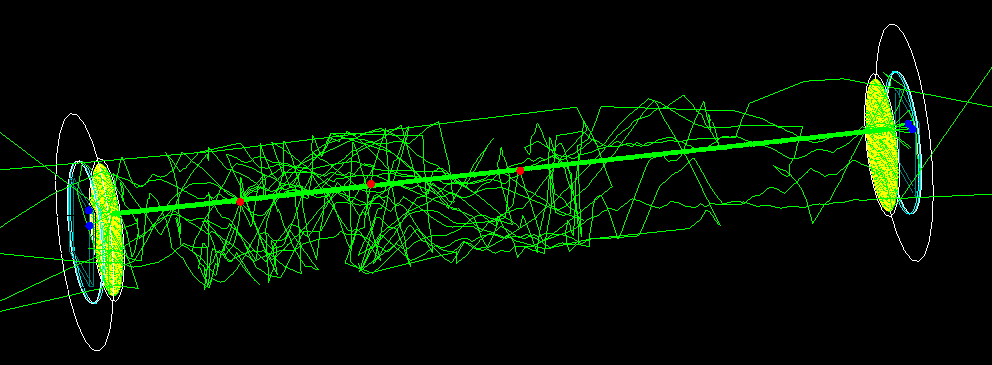
\includegraphics[scale=0.35]{6Simulations/62TRITIUMMonitor/621TRITIUMIFIC2/EventDetectedInTRITIUMIFIC2.png}
\caption{Tritium electron detected in the simulated TRITIUM-IFIC-2 prototype. The path of the optical photons is represented by green lines and the position in which they are absorbed is represented by red and blue dots for absorption in water or PMT, respectively.\label{fig:TritiumEventDetectedInSimulatedPrototype}}
\end{figure}
The different steps of the simulation were checked with variables such as production of tritium electrons, energy deposition in scintillating fibers and subsequent photon emission, the spatial distribution of generated events, number of detected events, etc. The distribution of the number of photons detected by photosensors per tritium event for the TRITIUM-IFIC-2 prototype is shown in Figure \ref{fig:SimulatedPhotonsDetected}. A maximum of $17$ photons is obtained for the TRITIUM-IFIC-2 prototype simulations, which is in agreement with the distribution of photons per tritium event measured experimentally, shown in Figure \ref{fig:PhotonsPerTritiumEventIFIC2}. The experimental distributions are lower than the simulations mainly in the range from $3$ to $8$ photons per event, probably due to imperfections not included in the simulations.

\begin{figure}[hbtp]
\centering
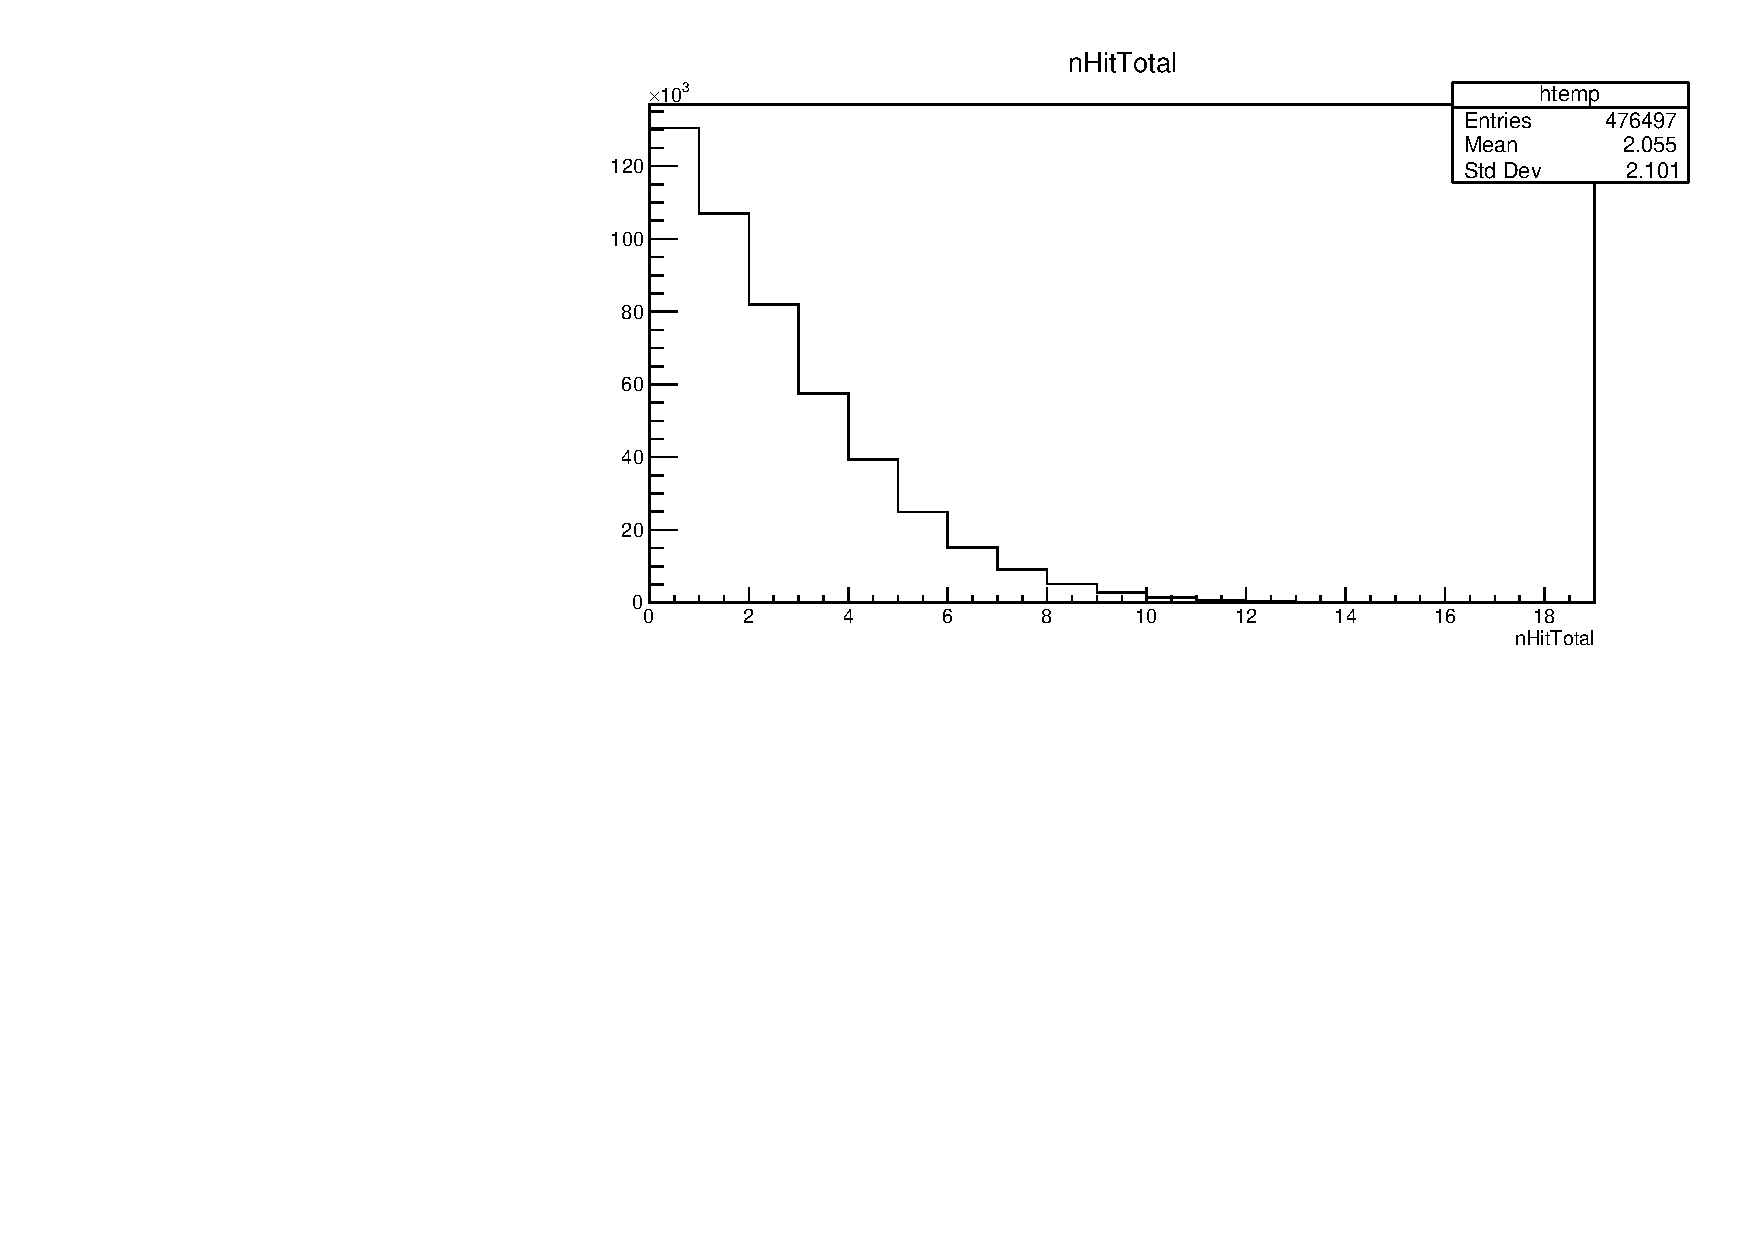
\includegraphics[scale=0.65]{6Simulations/62TRITIUMMonitor/621TRITIUMIFIC2/PhotonsDetected_simulation.pdf}
\caption{Photons detected by both PMTs per tritium event in the simulated TRITIUM-IFIC-2 prototype.\label{fig:SimulatedPhotonsDetected}}
\end{figure}

Activities from $100~\becquerel/\liter$ to $5~\kilo\becquerel/\liter$ for three months of data taking and an integration time of $10~\min$ were simulated. The simulation results are presented in Figure \ref{fig:1Det10Min250BqL}. A difference of $250~\becquerel/\liter$ in the activity is not distinguished due to the width of the distributions. To reduce the width, the statistics must be increased, either by increasing the integration time or the number of prototypes read out in parallel. To check the role of the integration time, distributions for integration times of $10~\min$, $30~\min$ and $60~\min$ were generated. The effect of increasing the integration time is to reduce the distribution width and to improve the activity resolution of the TRITIUM monitor as seen in Figure \ref{fig:1Det250BqLseveralTimes}. Differences as low as $250~\becquerel/\liter$ are clearly discriminated with only one TRITIUM-IFIC-2 module and an integration time of $60~\min$ which could still be considered a quasi-real time measurement. Similarly, these distributions are shown in Figure \ref{fig:SeveralDet250BqL10min} for $10~\min$ of integration time and for 1, 5 and 10 modules read out in parallel. A reduction of the distribution width with increasing number of modules is clearly visible in this figure, that improves the activity resolution of the detector. Differences of $250~\becquerel/\liter$ are clearly discerned with an integration time of $10~\min$ and 5 TRITIUM-IFIC-2 modules. The resolution, defined as
\begin{equation}
\text{Resolution(\%)}=\frac{\text{FWHM}}{\text{centroid}}\cdot{}100
\label{eq:Resolution}
\end{equation}
is plotted in Figure \ref{fig:Resolution}. It can be observed that the resolution improves with integration time and number of modules. The studied cases are summarized in Table \ref{tab:DifferentCasesOfTI2}.

\begin{figure}
\centering
    \begin{subfigure}[b]{0.7\textwidth}
    \centering
    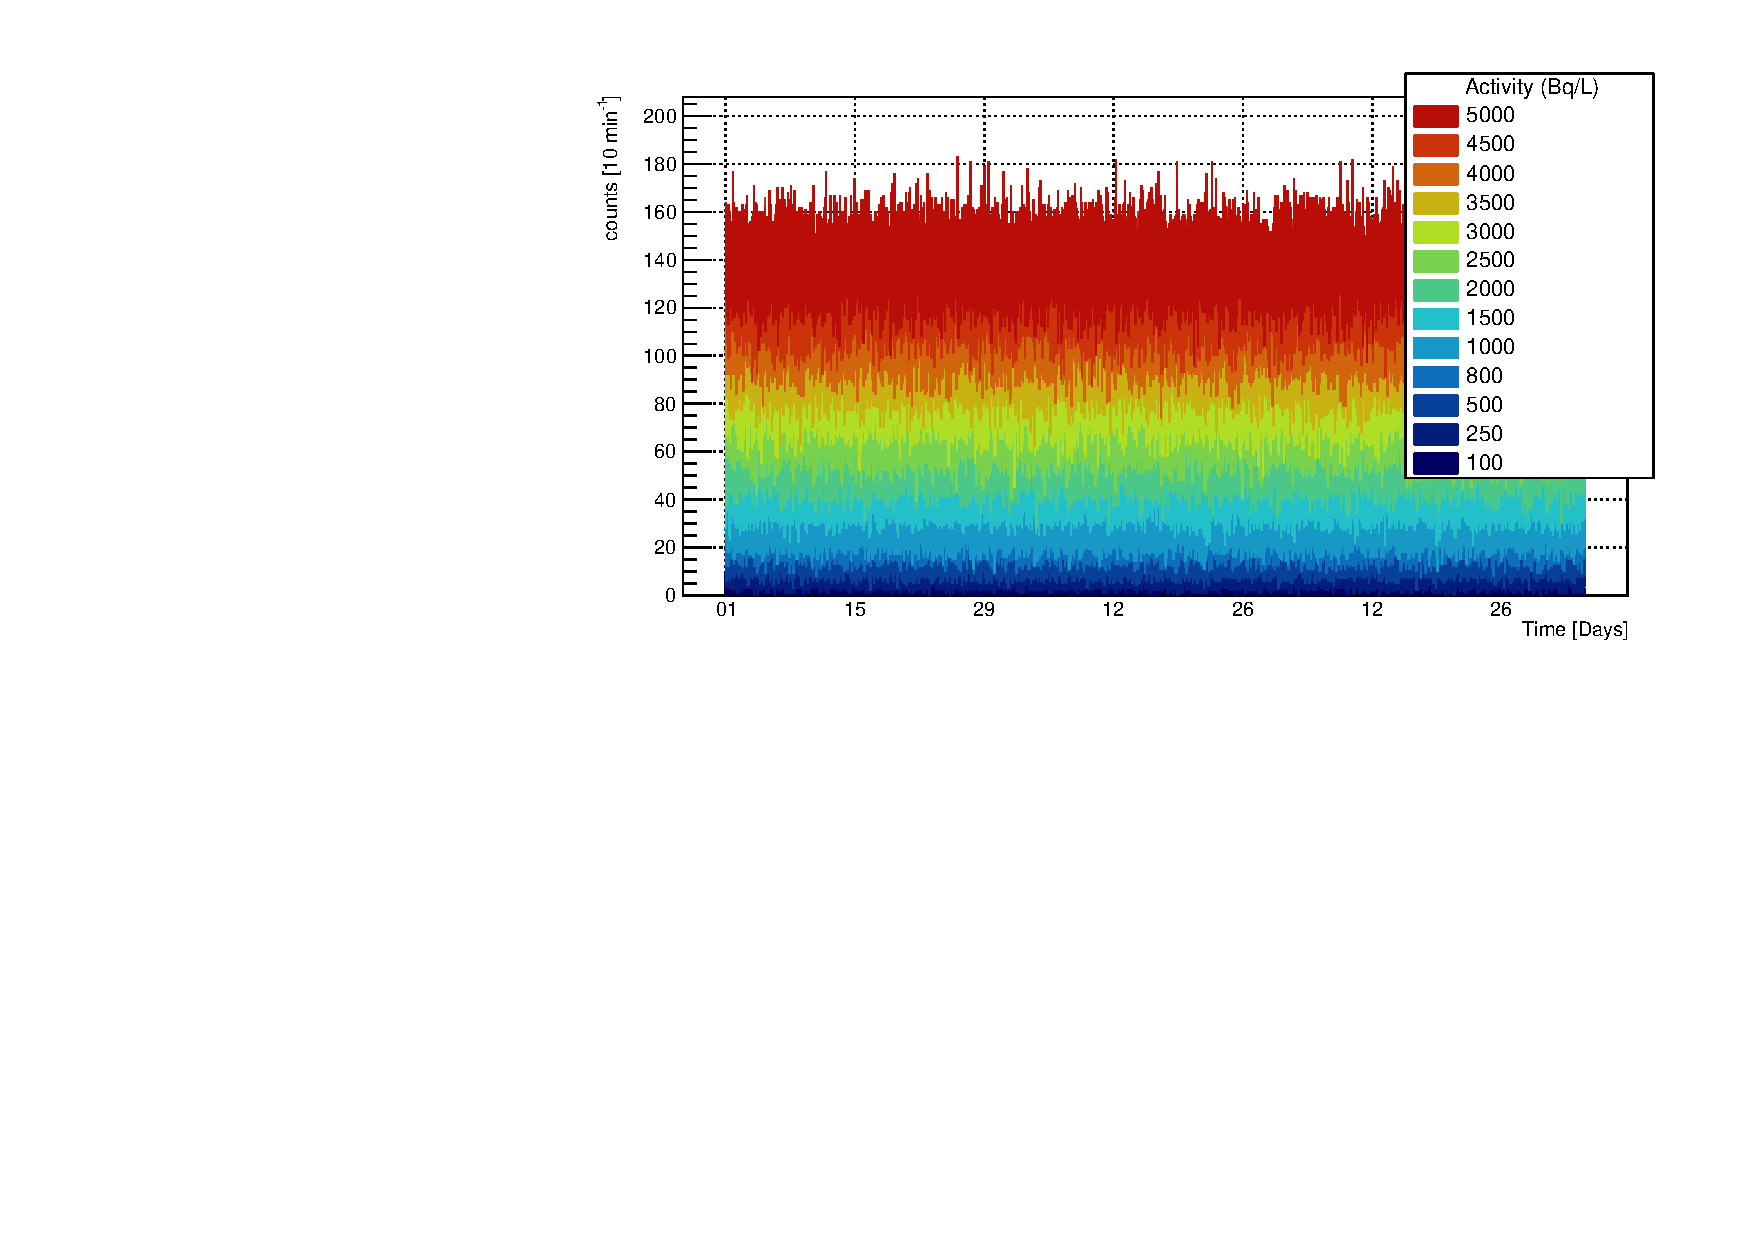
\includegraphics[width=\textwidth]{6Simulations/62TRITIUMMonitor/621TRITIUMIFIC2/RawData_1Det_10min_250BqL.pdf}  
    \caption{\label{subfig:RawData1Det10Min250BqL}}
    \end{subfigure}
    \hfill
    \begin{subfigure}[b]{0.7\textwidth}
    \centering
    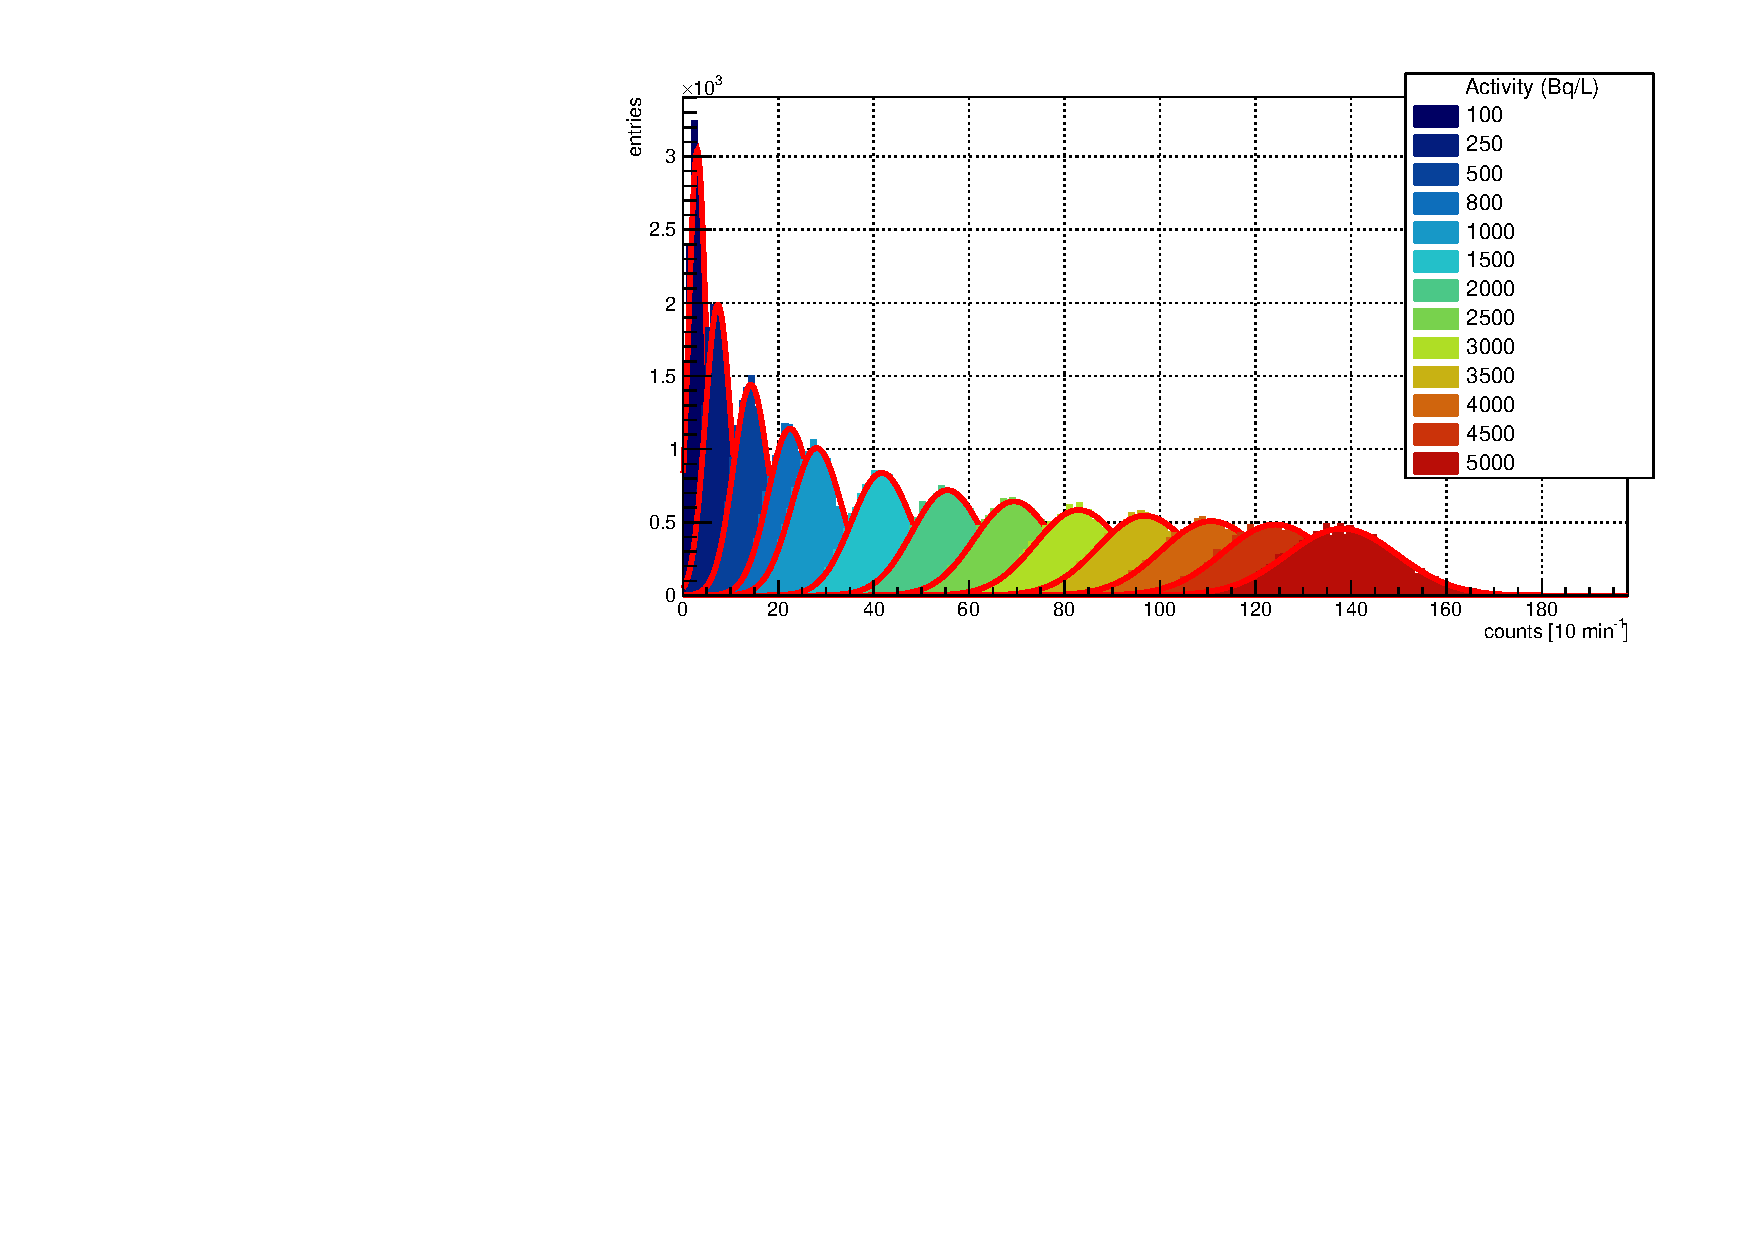
\includegraphics[width=\textwidth]{6Simulations/62TRITIUMMonitor/621TRITIUMIFIC2/Dist_1Det_10min_250BqL_and_Gaus.pdf}  
    \caption{\label{subfig:Dist1Det10Min250BqL}}
    \end{subfigure}
 \caption{a) Simulation of the tritium statistics measured with TRITIUM-IFIC-2 with an integration time of $10~\min$ during three months ($13248$ time bins for each activity). b) Distribution of counting statics versus activities.}
 \label{fig:1Det10Min250BqL}
\end{figure}

\begin{figure}
\centering
    \begin{subfigure}[b]{0.6\textwidth}
    \centering
    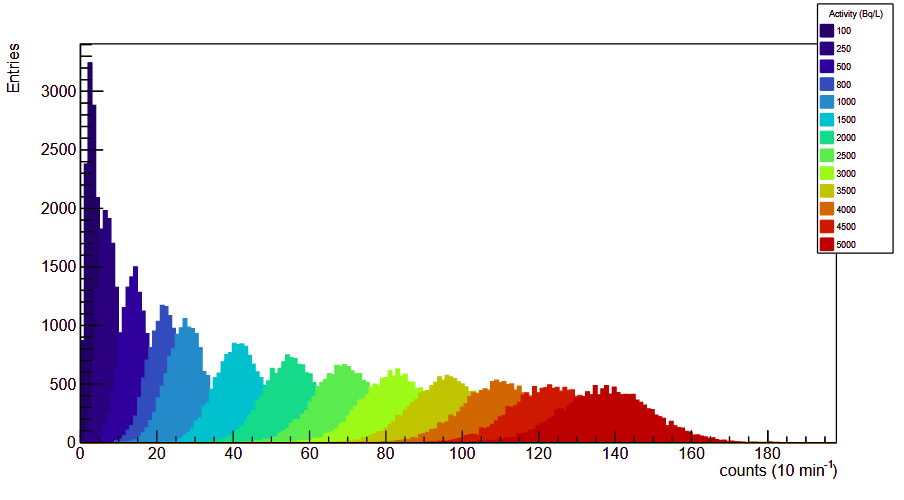
\includegraphics[width=\textwidth]{6Simulations/62TRITIUMMonitor/621TRITIUMIFIC2/Dist_1Det_10min_250BqL.png}  
    \caption{\label{subfig:1Det10min250BqLST}}
    \end{subfigure}
    \hfill
    \begin{subfigure}[b]{0.6\textwidth}
    \centering
    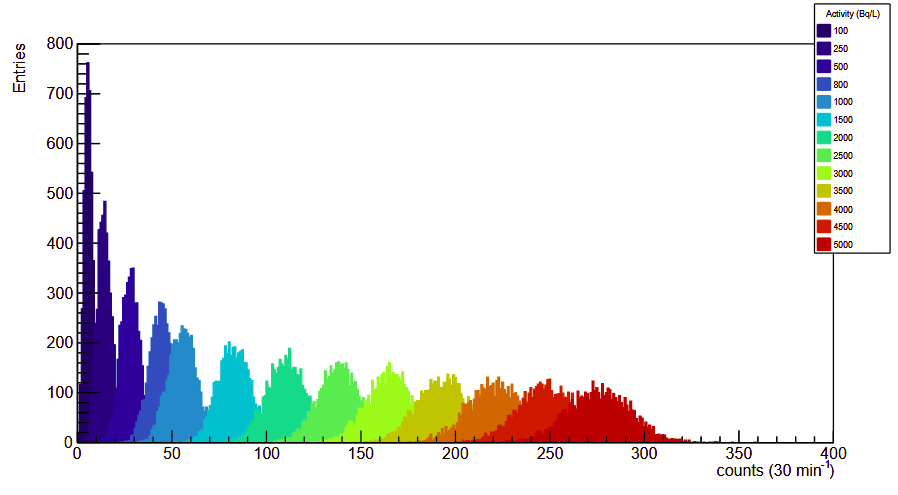
\includegraphics[width=\textwidth]{6Simulations/62TRITIUMMonitor/621TRITIUMIFIC2/Dist_1Det_30min_250BqL.png}  
    \caption{\label{subfig:1Det30min250BqLST}}
    \end{subfigure}
    \hfill
    \begin{subfigure}[b]{0.6\textwidth}
    \centering
    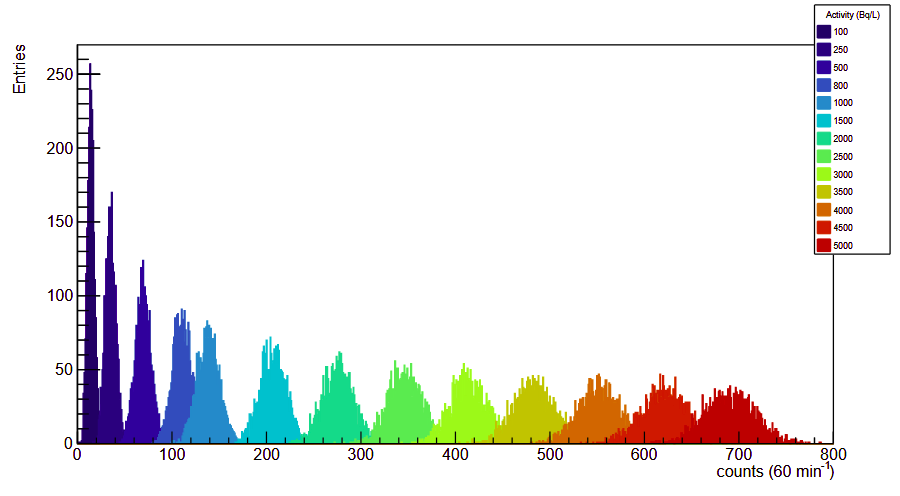
\includegraphics[width=\textwidth]{6Simulations/62TRITIUMMonitor/621TRITIUMIFIC2/Dist_1Det_60min_250BqL.png}  
    \caption{\label{subfig:1Det60min250BqLST}}
    \end{subfigure}
 \caption{Simulated tritium statistics obtained with a TRITIUM-IFIC-2 prototype versus tritium activities during three months of measurements and three different integration times: a)$10~\min$ ($13248$ bins), b) $30~\min$ ($4416$ bins) and c) $60~\min$ ($2208$ bins).}
 \label{fig:1Det250BqLseveralTimes}
\end{figure} 

\begin{figure}
\centering
    \begin{subfigure}[b]{0.6\textwidth}
    \centering
    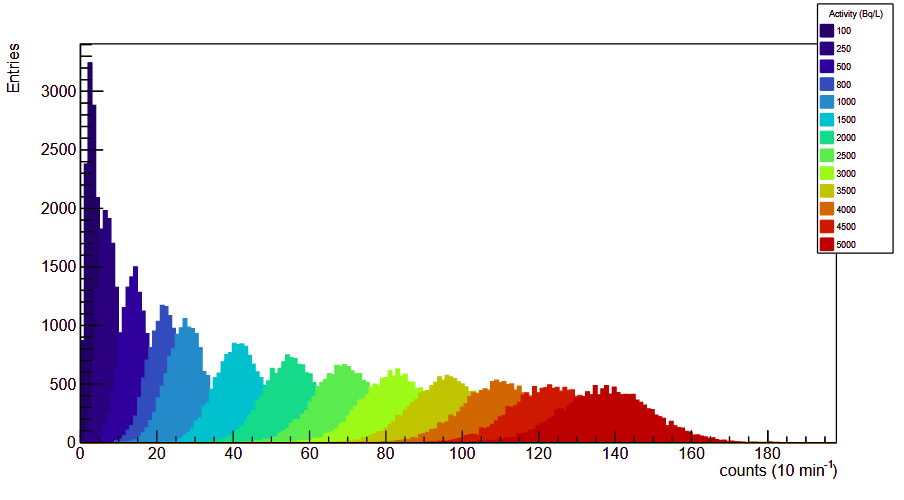
\includegraphics[width=\textwidth]{6Simulations/62TRITIUMMonitor/621TRITIUMIFIC2/Dist_1Det_10min_250BqL.png}  
    \caption{\label{subfig:1Det10min250BqLSD}}
    \end{subfigure}
    \hfill
    \begin{subfigure}[b]{0.6\textwidth}
    \centering
    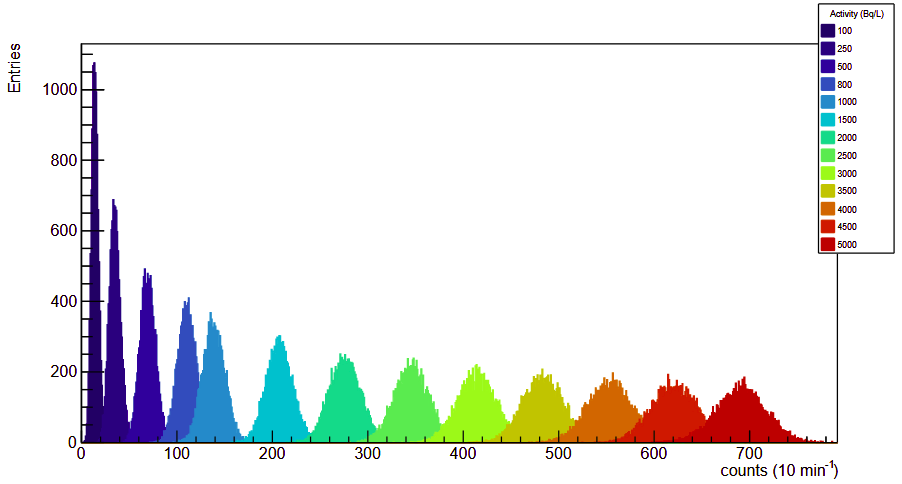
\includegraphics[width=\textwidth]{6Simulations/62TRITIUMMonitor/621TRITIUMIFIC2/Dist_5Det_10min_250BqL.png}  
    \caption{\label{subfig:5Det10min250BqLSD}}
    \end{subfigure}
    \hfill
    \begin{subfigure}[b]{0.6\textwidth}
    \centering
    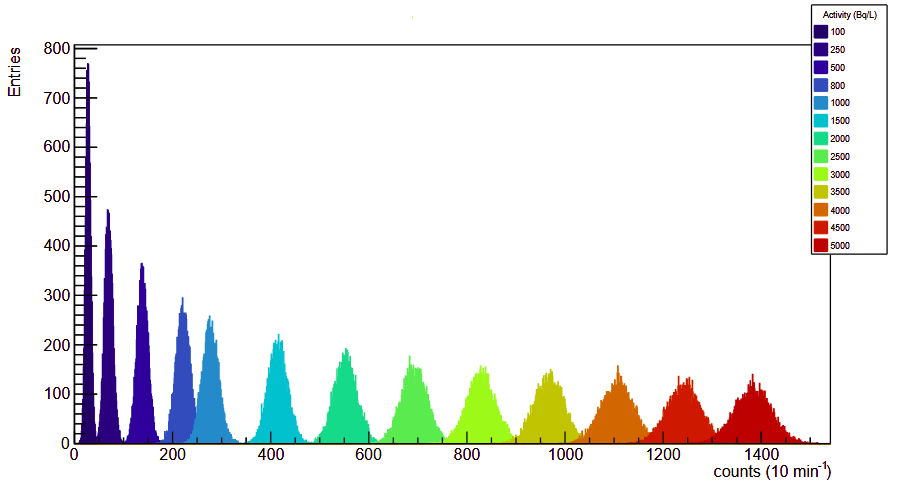
\includegraphics[width=\textwidth]{6Simulations/62TRITIUMMonitor/621TRITIUMIFIC2/Dist_10Det_10min_250BqL.png}  
    \caption{\label{subfig:10Det10min250BqLSD}}
    \end{subfigure}
 \caption{Simulated tritium statistics during three months with an integration time of $10~\min$ ($13248$ time bins) versus tritium activities for a) 1, b) 5 and c) 10 TRITIUM-IFIC-2 modules.}
 \label{fig:SeveralDet250BqL10min}
\end{figure}

\begin{figure}
\centering
    \begin{subfigure}[b]{0.75\textwidth}
    \centering
    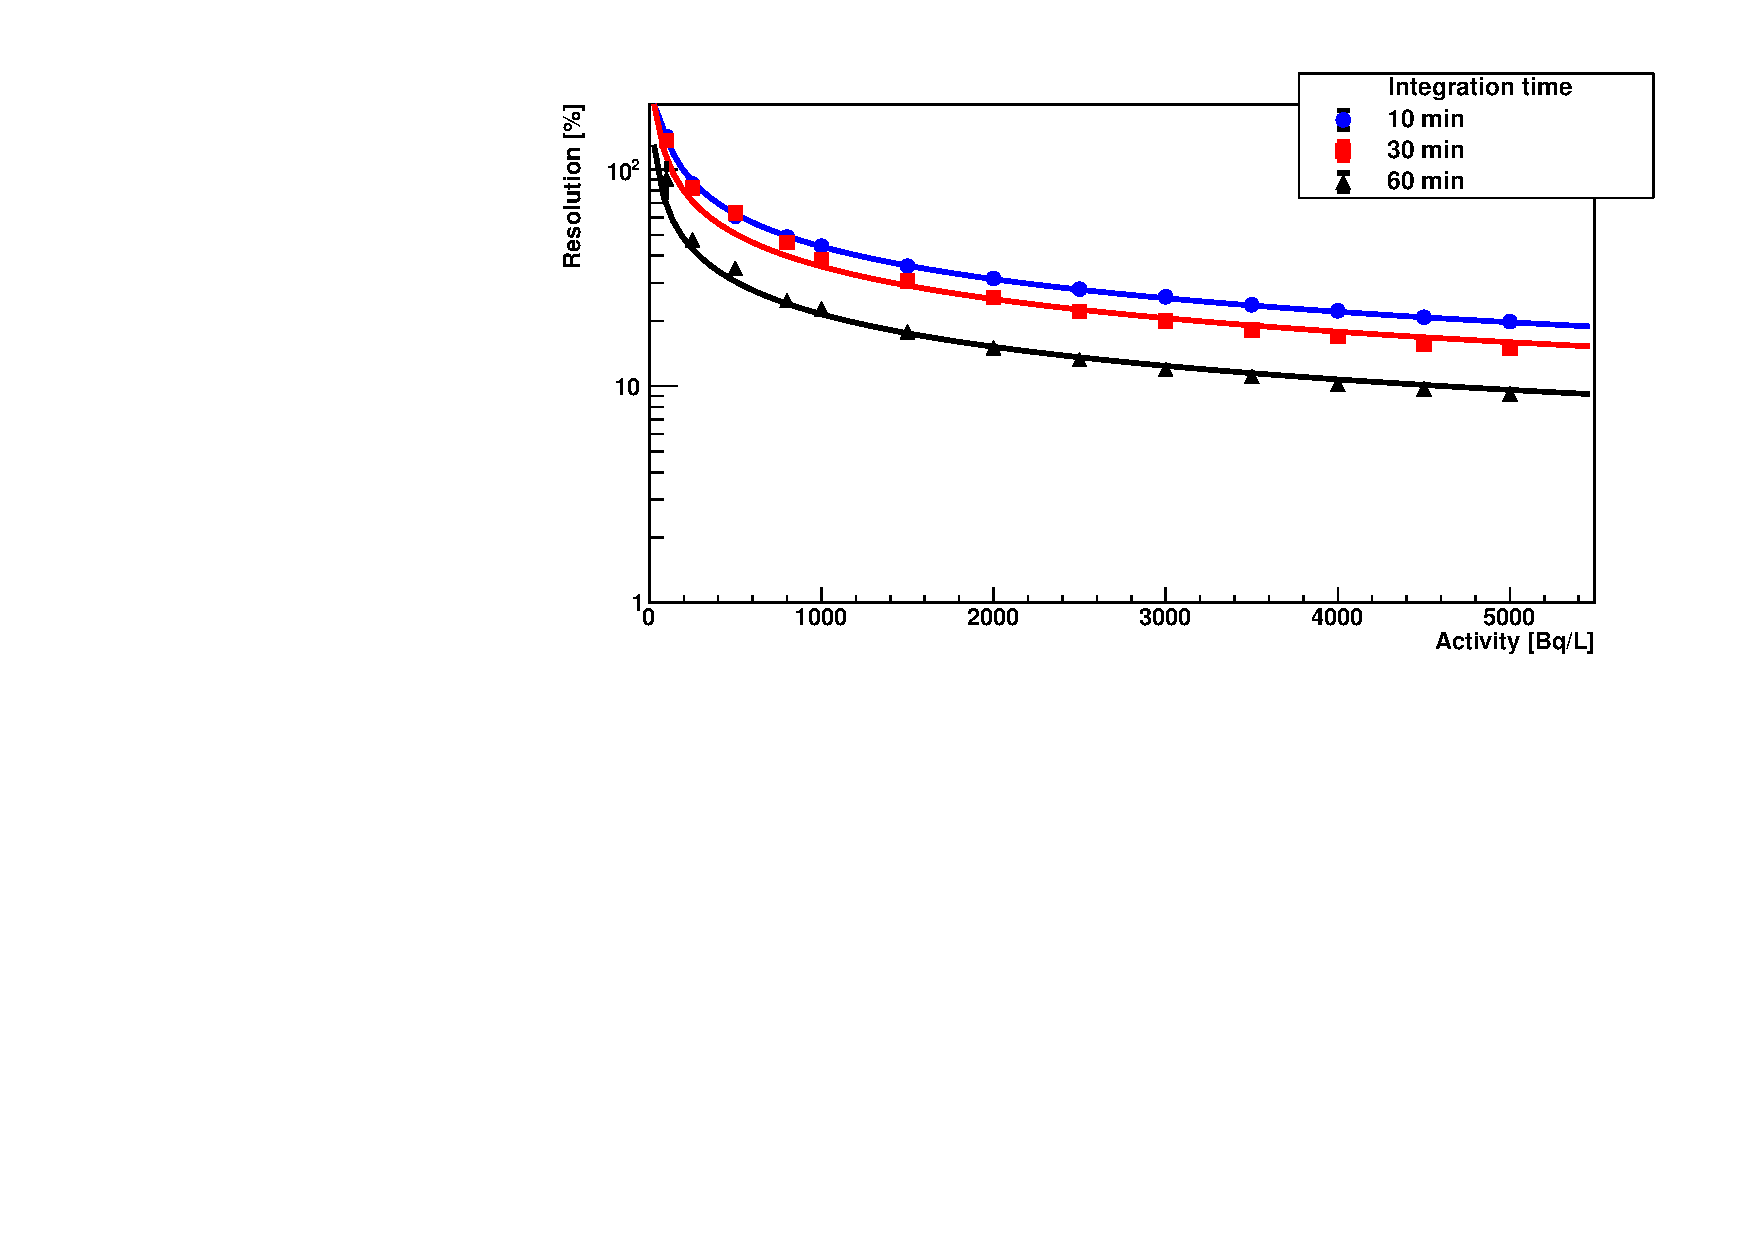
\includegraphics[width=\textwidth]{6Simulations/62TRITIUMMonitor/621TRITIUMIFIC2/Results_Several_Times.pdf}  
    \caption{\label{subfig:ResolutionvsIntegrationCoutingTime}}
    \end{subfigure}
    \hfill
    \begin{subfigure}[b]{0.75\textwidth}
    \centering
    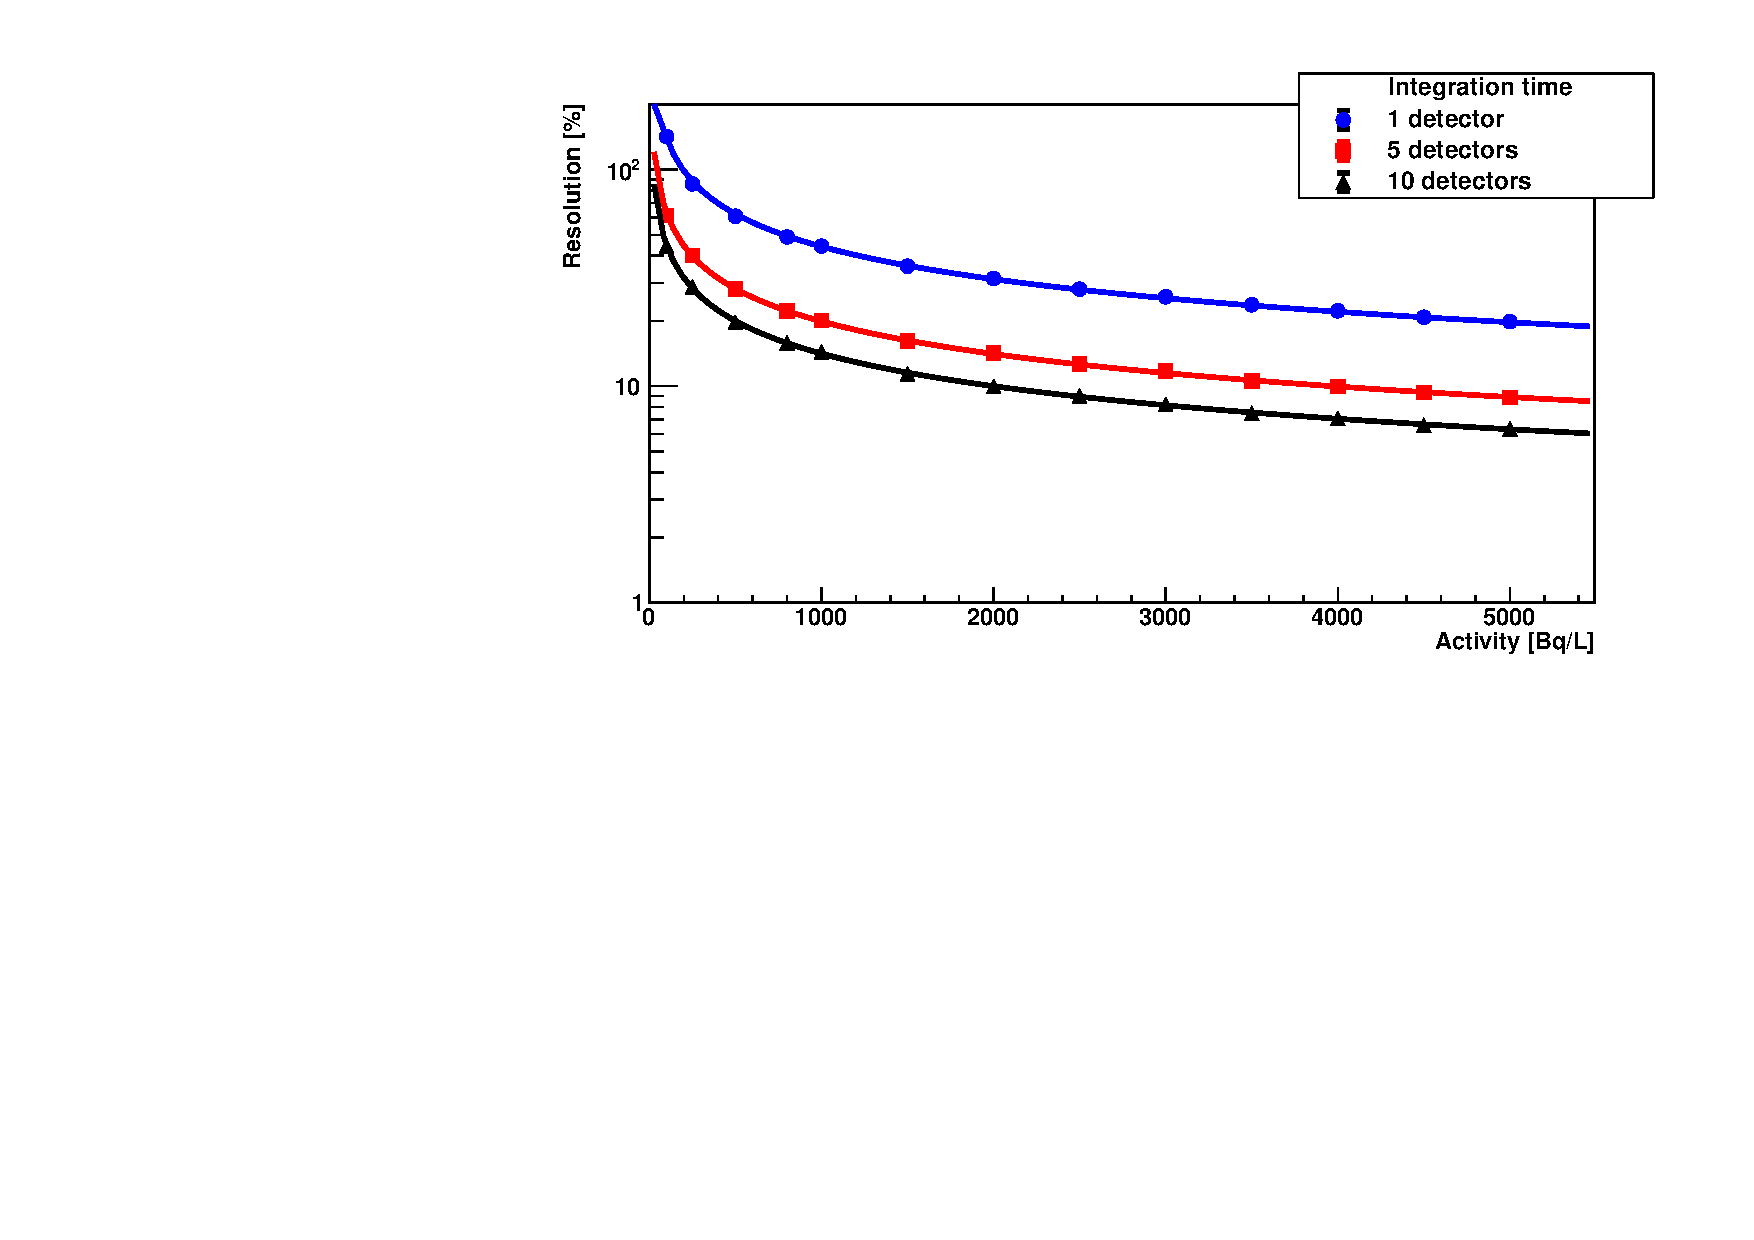
\includegraphics[width=\textwidth]{6Simulations/62TRITIUMMonitor/621TRITIUMIFIC2/Results_Several_Detectors.pdf}  
    \caption{\label{subfig:ResolutionvsNumberDetectors}}
    \end{subfigure}
 \caption{a) Resolution of TRITIUM-IFIC-2 versus tritium activity for different integration time using 1 TRITIUM-IFIC 2 module. b) Resolution of TRITIUM-IFIC-2 versus tritium activity for different number of modules and $10~\min$ integration time.}
 \label{fig:Resolution}
\end{figure}

\begin{table}[htbp]
\centering{}%
\begin{tabular}{lccc}
\toprule 
\# of modules & $10~\min$ & $30~\min$ & $60~\min$ \tabularnewline
\midrule
\midrule 
1 & $<1000~\becquerel/\liter$ & $500~\becquerel/\liter$ & $200~\becquerel/\liter$ \tabularnewline
5 & $200~\becquerel/\liter$ & $150~\becquerel/\liter$ & $100~\becquerel/\liter$ \tabularnewline
10 & $150~\becquerel/\liter$ & $100~\becquerel/\liter$ & $\approx 50~\becquerel/\liter$ \tabularnewline
\bottomrule
\end{tabular}
\caption{Difference in activity that can be resolved by TRITIUM-IFIC-2, for different integration times and different number of modules.}
\label{tab:DifferentCasesOfTI2}
\end{table}

The decision adopted by the TRITIUM collaboration is to install 5 TRITIUM-IFIC-2 modules with an integration time of $1~\hour$, that provide a MDA of $100~\becquerel/\liter$, as seen in Figure \ref{fig:MDATRITIUMmonitor}. With this configurations, differences of $100~\becquerel/\liter$ are expected to be resolved according to the table \ref{tab:DifferentCasesOfTI2}. 

%Three TRITIUM-IFIC-2 modules are planned to be installed in Arrocampo dam as soon as possible, which will be used to detect and solve prossible problems when several TRITIUM modules are read out in parallel. In addition, two other TRITIUM-Aveiro prototypes are being built and will be installed soon, to be read out in parallel with the one currently installed.

%Se ha realizado un ajuste lineal del centroide de las gaussianas de los ajustes (y su anchura como error) frente a la actividad usada. El rango utilizado en este caso ha sido mucho mayor debido a

%Tritium detection was studied using only one TRITIUM-IFIC-2 prototype, throguh the simulation of various activities of tritiated water. The integration count time used was $10~\min$ and continuous use of the detector during 3 months was simulated for each activity studied.


%PEORES RESULTADOS SIMULADOS QUE CON AVEIRO PERO MEJORES EXPERIMENTALMENTE. La diferencia debe de estar en que uno usa fibras pulida y limpiadas y el otro no.

%PREPARAR EN BACK UP EN LA PRESENTACIÓN EL CASO PARA 3 DETECTORES, YA QUE SERÁ NUESTRO CASO.














%The simulation of the Tritium-Aveiro prototype is similar to this since the design of both detectors are quite similar. There are two main difference between both simulated prototypes:

%\begin{enumerate}

%\item{} The diameter of the fibers used, which is $1~\mm$ for Tritium-IFIC-2 prototype and $2~\mm$ for Tritium-Aveiro prototype. As the internal volume of the PTFE vessel is filled, this difference imply a difference number of the scintillating fibers used, causing a difference in the signal-background ratio.

%\item{} The photosensors used since, although both are PMTs, the model of the used PMTs is different and it cause a different active area readout, affecting to the tritium detection efficiency. 

%\end{enumerate}